\documentclass[14pt, a4paper]{article}
\usepackage[T2A]{fontenc}
\usepackage[utf8]{inputenc}
\usepackage[russian]{babel}
\usepackage[left=3cm, right=1.5cm, top=2cm, bottom=2cm]{geometry}
\usepackage{indentfirst}
\usepackage{microtype}
\usepackage{array}
\usepackage{xcolor}
% \usepackage{times}
\usepackage{tempora}
\usepackage{ulem}
\usepackage{setspace}
\usepackage{amsmath}
\usepackage{booktabs}
\usepackage{graphicx}
\usepackage{float}
\usepackage{listings}
\graphicspath{{reports/figures/}{figures/}}
\lstset{basicstyle=\ttfamily\small, breaklines=true, columns=fullflexible, frame=single, keepspaces=true}
\pagestyle{empty}

\makeatletter
\renewcommand\section{\@startsection {section}{1}{\parindent}%
  {-3.5ex \@plus -1ex \@minus -.2ex}%
  {0.5ex}%
  {\normalfont\Large\bfseries}}
\renewcommand\tableofcontents{%
  \begin{center}\Large\bfseries\contentsname\end{center}%
  \@starttoc{toc}%
}
\renewcommand*\l@section{\@dottedtocline{1}{0em}{1.5em}}
\makeatother

\begin{document}
\onehalfspacing

\begin{center}
    \textbf{ФЕДЕРАЛЬНОЕ ГОСУДАРСТВЕННОЕ АВТОНОМНОЕ ОБРАЗОВАТЕЛЬНОЕ} \\
    \textbf{УЧРЕЖДЕНИЕ ВЫСШЕГО ОБРАЗОВАНИЯ} \\
    \textbf{«МОСКОВСКИЙ АВИАЦИОННЫЙ ИНСТИТУТ} \\
    \textbf{(НАЦИОНАЛЬНЫЙ ИССЛЕДОВАТЕЛЬСКИЙ УНИВЕРСИТЕТ)»}
\end{center}

\begin{center}
    \bfseries Институт №8 «Компьютерные науки и \\
    \bfseries прикладная математика» \\
    \bfseries Кафедра 806 «Вычислительная математика \\
    \bfseries и программирование»
\end{center}

\vspace{3cm}

\begin{center}
    \Large\bfseries Отчет \\
    \vspace{0.5cm}
    \mdseries по лабораторной работе №4.1
\end{center}

\vfill

\noindent
\hfill
\begin{tabular}{ll}
Группа:       & М8О-307Б-21 \\
Студент:      & М. С. Ивченко \\
Преподаватель:& доц. В. В. Киндинова \\
Оценка:       & \underline{\makebox[3cm][c]{}} \\ [0.2cm]
Дата:         & \underline{\makebox[3cm][c]{}}
\end{tabular}

\vfill

\begin{center}
    Москва \\
    2026
\end{center}

\newpage

\setcounter{tocdepth}{2}
\tableofcontents
\newpage

\section*{Тема}
\addcontentsline{toc}{section}{Тема}
Цель данной лабораторной работы -- исследовать численные методы решения задачи Коши для обыкновенных дифференциальных уравнений. Методы Эйлера, Рунге-Кутты и Адамса позволяют проследить эволюцию решения по сетке и сравнить простые и более точные схемы интегрирования.

\section*{Задание}
\addcontentsline{toc}{section}{Задание}
Реализовать методы Эйлера, Рунге-Кутты и Адамса 4-го порядка в виде программ, задавая в качестве входных данных шаг сетки $h$. С использованием разработанного программного обеспечения решить задачу Коши для ОДУ 2-го порядка на указанном отрезке. Оценить погрешность численного решения с использованием метода Рунге-Ромберга и путем сравнения с точным решением.

\section*{Теория}
\addcontentsline{toc}{section}{Теория}
Задача Коши для ОДУ второго порядка содержит уравнение и начальные условия для функции и ее производной. Чтобы применять стандартные одношаговые методы, уравнение второго порядка сводится к системе первого порядка заменой
\[
    z_1=y,\qquad z_2=y'.
\]
Тогда $z_1'=z_2$, а $z_2'$ выражается из исходного уравнения. Векторное решение $z=(z_1,z_2)^T$ ищется на сетке $x_i=x_0+ih$.

Метод Эйлера использует явный шаг
\[
    z_{k+1}=z_k+h f(x_k,z_k),
\]
то есть заменяет решение касательной в начале шага. Метод прост, но имеет первый порядок точности, поэтому ошибка заметно уменьшается только при сильном измельчении сетки.

Метод Рунге--Кутты 4-го порядка комбинирует четыре оценки наклона: в начале шага, в двух серединах и в конце. Итоговое приращение является взвешенным средним этих наклонов, поэтому локальная ошибка имеет порядок $O(h^5)$, а глобальная -- $O(h^4)$.

Метод Адамса 4-го порядка является явным многошаговым методом. Он использует значения правой части в четырех предыдущих узлах:
\[
    z_{k+1}=z_k+\frac{h}{24}\left(55f_k-59f_{k-1}+37f_{k-2}-9f_{k-3}\right).
\]
Первые точки для него обычно получают методом Рунге--Кутты, после чего многошаговая формула продолжает расчет.

Для оценки ошибки применяется сравнение с точным решением, если оно известно, и метод Рунге--Ромберга. При двух расчетах с шагами $h$ и $h/r$ погрешность метода порядка $p$ оценивается как
\[
    \frac{y_{h/r}-y_h}{r^p-1}.
\]

\begin{lstlisting}[language=Python]
k1 = h * f(x[i], y[i])
k2 = h * f(x[i] + h/2, y[i] + k1/2)
k3 = h * f(x[i] + h/2, y[i] + k2/2)
k4 = h * f(x[i] + h, y[i] + k3)
y[i + 1] = y[i] + (k1 + 2*k2 + 2*k3 + k4) / 6
\end{lstlisting}

\section*{Ход лабораторной работы}
\addcontentsline{toc}{section}{Ход лабораторной работы}
Решалась задача Коши
\[
    y''+y'\tan x-y\cos^2x=0,
    \qquad y(0)=2,\quad y'(0)=0,
\]
на $[0,1]$ с шагом $h=0.1$. Точное решение:
\[
    y=e^{\sin x}+e^{-\sin x}.
\]
\begin{table}[H]
\centering
\begin{tabular}{lrrr}
\toprule
Метод & $y(1)$ & $y'(1)$ & $|y_{exact}(1)-y(1)|$\\
\midrule
Эйлер & 2.7260761990 & 1.1097071116 & 0.0247765764\\
Рунге--Кутта 4 & 2.7508530900 & 1.0204605453 & 0.0000003147\\
Адамс 4 & 2.7505525844 & 1.0199229472 & 0.0003001909\\
\bottomrule
\end{tabular}
\caption{Сравнение значений в конце отрезка.}
\end{table}

\begin{figure}[H]
    \centering
    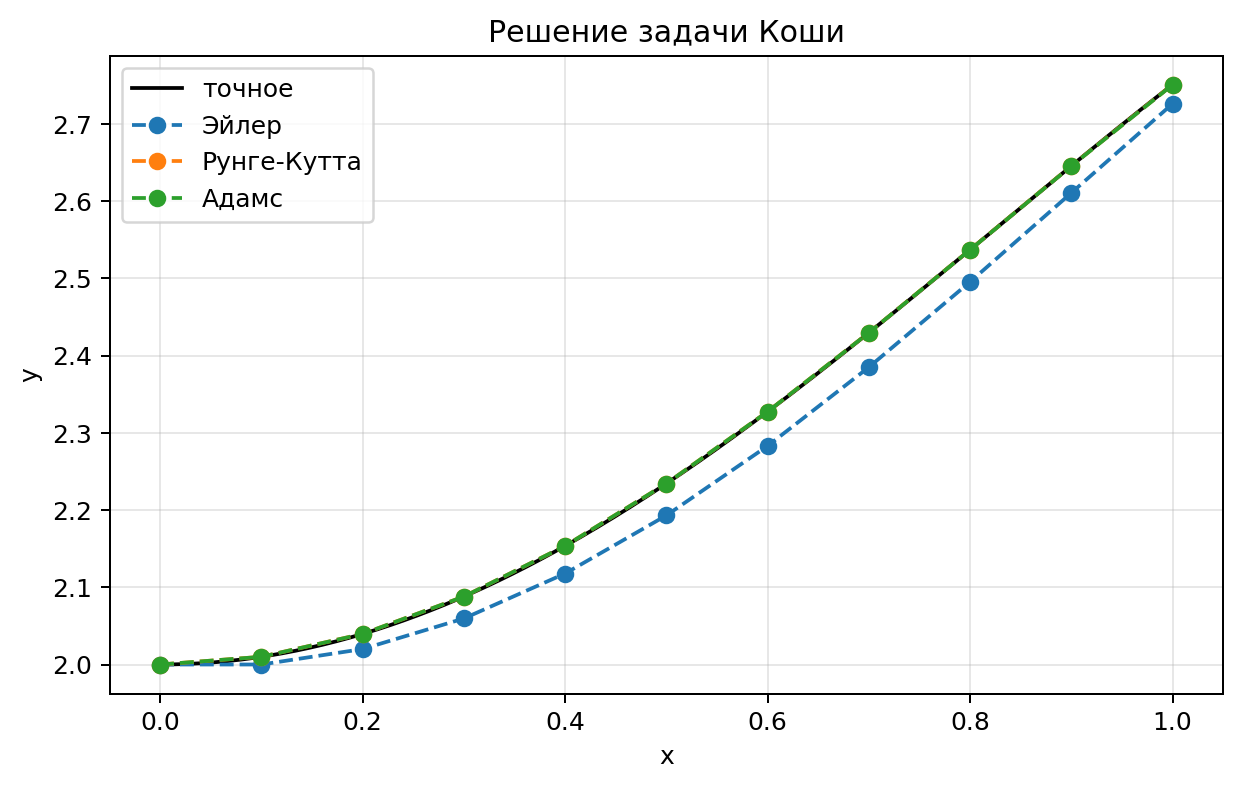
\includegraphics[width=0.86\textwidth]{lab4_1_solutions.png}
    \caption{Численные и точное решения задачи Коши.}
\end{figure}

\begin{figure}[H]
    \centering
    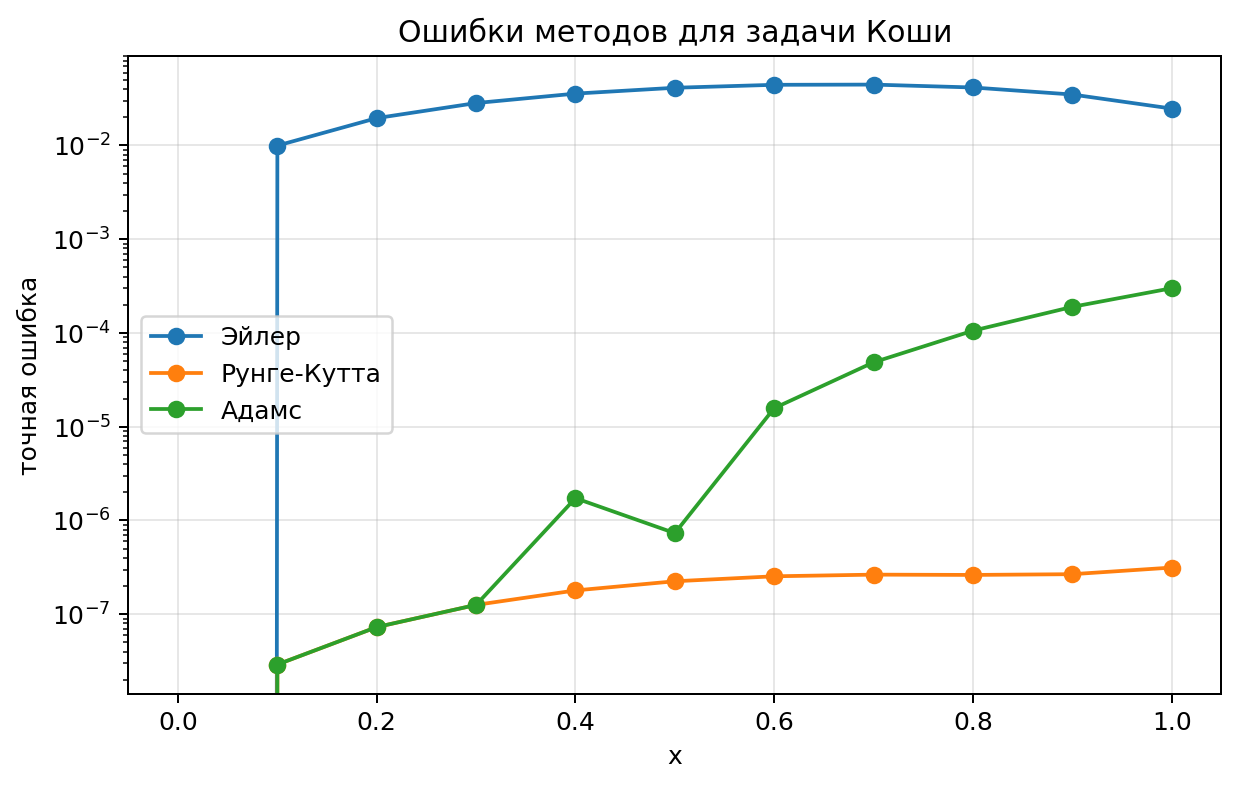
\includegraphics[width=0.86\textwidth]{lab4_1_errors.png}
    \caption{Ошибка относительно точного решения на сетке.}
\end{figure}

\section*{Выводы}
\addcontentsline{toc}{section}{Выводы}
На заданном шаге наименьшую ошибку показал метод Рунге--Кутты 4-го порядка. Метод Адамса также имеет четвертый порядок, но его точность зависит от стартовых значений и накопления ошибки в многошаговой формуле; метод Эйлера ожидаемо оказался самым грубым.

\end{document}
